% The testflow support page is at:
% http://www.michaelshell.org/tex/testflow/



\documentclass[conference]{IEEEtran}

% *** CITATION PACKAGES ***
%
\usepackage{cite}

% *** GRAPHICS RELATED PACKAGES ***
%
\ifCLASSINFOpdf
 \usepackage[pdftex]{graphicx}
  % declare the path(s) where your graphic files are
  % \graphicspath{{../pdf/}{../jpeg/}}
  % and their extensions so you won't have to specify these with
  % every instance of \includegraphics
  % \DeclareGraphicsExtensions{.pdf,.jpeg,.png}
\else
  % or other class option (dvipsone, dvipdf, if not using dvips). graphicx
  % will default to the driver specified in the system graphics.cfg if no
  % driver is specified.
  % \usepackage[dvips]{graphicx}
  % declare the path(s) where your graphic files are
  % \graphicspath{{../eps/}}
  % and their extensions so you won't have to specify these with
  % every instance of \includegraphics
  % \DeclareGraphicsExtensions{.eps}
\fi

% *** MATH PACKAGES ***
%
\usepackage{amsmath}

\interdisplaylinepenalty=2500

% *** SPECIALIZED LIST PACKAGES ***
%
\usepackage{algorithmic}


% *** ALIGNMENT PACKAGES ***
%
%\usepackage{array}

% *** SUBFIGURE PACKAGES ***
%\ifCLASSOPTIONcompsoc
%  \usepackage[caption=false,font=normalsize,labelfont=sf,textfont=sf]{subfig}
%\else
%  \usepackage[caption=false,font=footnotesize]{subfig}
%\fi

% *** FLOAT PACKAGES ***
%
%\usepackage{fixltx2e}

%\usepackage{stfloats}

% *** PDF, URL AND HYPERLINK PACKAGES ***
%
\usepackage{url}

% correct bad hyphenation here
\hyphenation{op-tical net-works semi-conduc-tor}


\begin{document}
\title{Resource Aware LDPC Decoder Algorithm on ARM and GPU of Mobile Devices}

% author names and affiliations
% use a multiple column layout for up to three different
% affiliations
\author{\IEEEauthorblockN{Roohollah Amiri}
\IEEEauthorblockA{Department of Electrical and\\Computer Engineering\\
Boise State University\\
Email: roohollahamiri@boisestate.edu}
\and
\IEEEauthorblockN{Hani Mehrpouyan}
\IEEEauthorblockA{Department of Electrical and\\Computer Engineering\\
Boise State University\\
Email: hanimehrpouyan@boisestate.edu}
\and
\IEEEauthorblockN{Inanc Senocak}
\IEEEauthorblockA{Department of Mechanical Engineering\\
Boise State University\\
Email: senocak@boisestate.edu}
}

% use for special paper notices
%\IEEEspecialpapernotice{(Invited Paper)}


% make the title area
\maketitle

% As a general rule, do not put math, special symbols or citations
% in the abstract
\begin{abstract}
Low Density Parity Check(LDPC) code is an efficient way of communication and is beeing largely used in mobile communication. With the wide usage and having computational intensivity of LDPC decoders, there has been a lot of effort to reduce decoder's complexity through algorithm optimization and parallel implementation. Recent improvements in mobile processors's architectures has made it exclusively reachable to have a real-time decoder based on a software solution. Knowing this capability, low profile GPU based decoders has been introduced that are capable of reaching high throughput by low latency. On the other hand recently there has been some work that has used ARM NEON SIMD unit with promising throughput and latency. What this works miss is that a mobile processor that is used in a smart phone should support a lot of task and we can not allocate all resources to decoding prcesses. In this paper we propose a heterogeneous LDPC decoder that uses both ARM and GPU Processors of a mobile device to reach real-time effieciency. The different stages of decoder processes has been allocated to ARM and GPU based on an optimization solution. 
\end{abstract}

% no keywords

\IEEEpeerreviewmaketitle



\section{Introduction}
% no \IEEEPARstart
% LDPC , Usages, Complexity
Originally proposed by Robert Gallager in 1962 \cite{art_gallager} and rediscovered by MacKay and Neal in 1996 \cite{art_macKay} Low Density Parity Check (LDPC) codes have been adopted by a wide range of applications including many communication system standards such as WiFi(IEEE 802.11n), 10 Gbit Ethernet (IEEE 802.3an), WiMAX (IEEE 802.16e), and DVB-S2. Recently, Chung and Richardson \cite{art_shannon} showed that the LDPC code can approach the Shannon limit to within 0.0045 dB. However, the drawback of high correcting efficiency comes from its decoding computation complexity \cite{art_ldpc_cpu1} and to date there exist no known mathematical tools to accurately evaluate their performance. Thus, a resort is typically made to simulations using computers or dedicated hardware \cite{art_memory_coalesced}.

% Initial implementation
LDPC decoding algorithms are compute-intensive and need powerful computer architecture to convey low latency and high decoding rate which caused to be initially implemented using application-specific integrated circuits(ASIC) and field-programmable gate array(FPGA) circuits \cite{art_ldpc_OpenCl_1}. However, their high speed often comes at a price of high developement cost and low programming flexibility \cite{art_convolutional} and it is very challenging to design decoder hardware that supports various standards and multiple data rates \cite{art_cuda_openmp}. On the other hand, iterative LDPC decoding schemes based on the sum-product algorithm (SPA) can fully be parallelized, leading to high-speed decoding \cite{art_shannon}. For these reasons, designers have recently focused on software implementations of LDPC decoders on multi/many-core devicdes \cite{art_massively} to achieve requirements through Software Defined Radio (SDR) Systems.

% Availabe multi-core architectures
As in terms of multicore architectures, researchers have used CPUs \cite{art_cpu_gpu, art_ldpc_cpu0}, GPUs \cite{art_memory_coalesced, art_massively, art_optimize_0}and ARM \cite{art_ldpc_cpu0, art_neon} architectures to develop high throughput, low latency SDR systems. 

%CPUs
In microarchitectures, increasing clock frequencies to obtain peorformance has reached a limit, so to hold this increase, other techniques based on parallel processing is being investigated \cite{art_ldpc_cpu1}. Todays' multicore architectures support SIMD (Single Instruction Multiple Data), SPMD(Single Programm Multiple Data) and SIMT(Single Instruction Multiple Threads). The general purpose multicore processors replicate a single core in a homogeneous way, typically with a x86 instruction set, and provide shared memory hardware mechanisms\cite{art_massively}. They can be programmed at a high level by using different software technologies \cite{art_multicore_techs}. OpenMP \cite{art_openMp_book} provides an effective and relatively straightforward approach for programming general-purpose multicores. On the other hand newer microarchitectures are trying to provide larger SIMD units for vector processing like SSE, AVX and AVX2 \cite{art_intel_sse} on Intel Architectures. In \cite{art_ldpc_cpu1}, the authors have used Intel SSE/AVX2 SIMD Units to effieciently implement a high throughput LDPC decoder. In \cite{art_cuda_openmp}, OpenMP is used to generate address patterns with parity check H-matrix.

%GPUs
Mainly due to the demands for visualization technology in the games industry, the performance of graphics processing units (GPUs) has undergone increasing performances over the last decade. With many cores driven by a considerable memory bandwidth, recent GPUs are targeted for computationally intensive, multithreaded, highly parallel computation, and researchers in high-performance computing fields are applying GPUs to general-purpose applications (GPGPU) \cite{art_gpu_0,art_cuda_openmp, art_memory_coalesced, art_ldpc_OpenCl, art_optimize_0, art_layered1}. They have used Compute Unified Device Architecture (CUDA)
from NVIDIA \cite{website_cuda} and Open Computing Language (OpenCL) platforms to develop LDPC Decoders.

%ARMs and NEON
Due to large computing capacity of multicore devices, software LDPC decoders have met the required throughputs of communication standards, although power consumption of x86 and GPU devices is incompatible with most of the embedded systems \cite{art_neon}. To solve this issue, ARM-based SDR systems have been prposed in recent years \cite{art_neon, art_ldpc_cpu0, art_ldpc_OpenCl_1} with goal of a SDR LDPC decoder that provides high through, low latency on a low-power embedded system. The authors in \cite{art_neon} have used ARM Processors's NEON SIMD and SIMT programming models to implement to implement a horizontal layered-based decoder that is based on parallel decoding of a low set of frames. This approach allows reaching high throughput while maintaining low-latency. Due to restrictions in an embedded system, using all resources of the system is a crucial task. Recent works in SDR LDPC embedded systems are missing the fact that todays mobile devices have powerful CUDA enabled GPUs. This paper has prposed a new algorithm that exploits ARM NEON SIMD Units and GPU together to reach a high throughput, low latency LDPC decoder. The main specification of the algorithm is that is devides processing task between system's resources. 

\section{LDPC codes and their Decoding Processes}

Many works as in \cite{art_massively, art_ldpc_cpu0,art_ldpc_OpenCl_1,art_gpu_0} focused on mapping LDPC decoders on multicore architectures. Most of these works are based on the standard Two-Phase Message Passing (TPMP) schedule described in \cite{art_massively}. This algorithm works in two phases. In the first phase, all the variable nodes send messages to their neighboring parity check nodes, and in the second phase the parity check nodes send messages to their neighboring variable nodes. Due to transcendental operations and relying of Sum-Product algorithm to the estimation of noise standard deviation, in practice Min-Sum (MS) variants are prefered by designers \cite{art_neon}. More efficient layered schedules, such horizontal layered-based decoding algorithm, allow updated imformation to be utilized more quickly in the algorithm thus speeding up the decoding\cite{art_layered0, art_layered1}. In fact, the parity check matrix can be viewed as a layered graph decoded sequentially. Thw work in \cite{art_gpu_0} has applied a form of layered belief propogation to irregular LDPC codes to reach 2x faster convergence in a given error rate.By using this methos they have reduced memory bits usage by 45-50\%. The major limitation of layered algorithm is its irregular memory access although it is composed of a single loop kernel composed to two sequential kernels in standard algorithms. To solve the irregular memory access a data interleaving/deinterleaving process is bein used before and after the decoding process \cite{art_gpu_0, art_neon}.

In this paper the interleaving/deinterleaving process is done ny using ARM Vector processing units and frame decoding is being done in GPU of a mobile device.

\section{Parallel Frame Processing}
The porposed LDPC decoder is implemented on Jetson TK1 SoCs which contains 4 Cortex-A15 processors. Each core includes a NEON SIMD unit. To achieve high throughput performance on such low-power embedded processors, the following programming model is exploited in the proposed LDPC decoder.

\begin{figure}[h]
\begin{centering}
\scalebox{0.4}{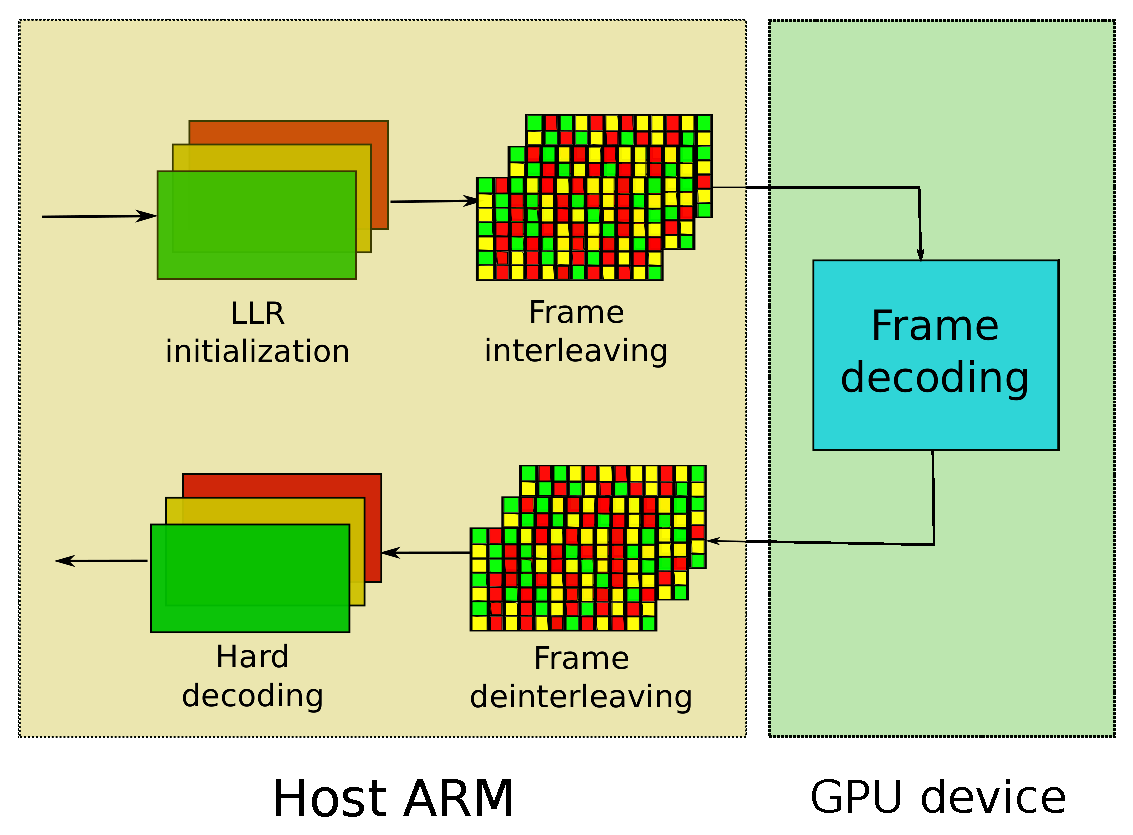
\includegraphics{structure.eps}}
\caption[width=.3\textwidth]{Proposed Setup for Heterogeneous LDPC decoding}
\label{fig_porposed_alg}
\end{centering}
\end{figure}

Typically, there are two ways to deliver messages in LDPC decoding. One is to use probabilities, and the other is to use log-likelihood ratios (LLRs). In general, using LLRs is favored since that allows us to replace expensive multiplication operations with inexpensive addition operations \cite{art_cuda_openmp}. So the host is in charge of Initialization of Check Nodes (CNS), Frame interleaving befor decoding and frame deinterleaving after decoding. From decoder point of view, host sends/receive data to/from the GPU device as the decoder. The GPU device is responsible for all CNs to Variable Nodes(VNs) computations that is done in one kernel (see figure \ref{fig_porposed_alg}). At the end of decoding, hard decision decodings are taken and decisions are sent back to the host.
SIMD programming model in host enables each processor core to interleave F frames in parallel with 8-bitxF the width in bits of SIMD unit. So there is C (number of host cores) set of F frame streams of data into GPU device. Each processor controls its own stream to GPU. On the GPU there are C similar kernel running. As long as the memory that is used in GPU is bigger than CxFx8-bits, there would be no problem in memory allocation. 



\section{Experimental Results}

The experiments were carried out by decoding LDPC codes using NVIDIA Tegra K1 Socs. The programs compiled with GCC-4.8 and CUDA 6.5. The TK1 is composed of 4 cortex-A15 ARM processors and one NVIDIA Kepler "GK20a" GPU with 192 SM3.2 CUDA cores. The host platform uses a GNU/Linux kernel 3.10.40-gdacac96. 

\section{Conclusion}
The conclusion goes here.

\newpage

\bibliographystyle{IEEEtran}
\bibliography{IEEEabrv,ldpcGpuTegra_bibliography}



% that's all folks
\end{document}


